%!TEX root = ../main.tex

In this section the measure of success and the scope of the method will be described. In terms of scope the aim of the method is to produce plausible lighting for Augmented Reality applications, and thus increase the sense of realism of the composed graphics. This does not mean that imagery that would for all practical purposes be indistinguishable from reality will be achieved. As said earlier, the non-matching lighting is only one of the problems with current AR graphics. In order to achieve complete realism all the other problems would have to be tackled as well, this includes occlusion from real objects as the most prominent one, but also the shadows of real objects not affecting the virtual ones at all. The method will also not attempt to improve other aspects of AR, such as tracking. The method comprises an offline and an online phase, offline being the acquisition of the 360 panorama and it's analysis for calculation; online is the actual rendering. It is also desirable and expected that the offline phase can be completed within a reasonable time frame on a mobile device, in terms of usability this should be no more than 1 minute.\newline
Since the final product is a graphic on a screen, an image, it's somewhat difficult to define a measure of success, due to the inherent subjective nature of image appreciation. It can be said that the method successfully converged if in the final image the synthetic objects are hard to tell from the real ones, if formed on a line on a still image. Hard to tell meaning that some scrutiny and reflection is necessary when looking at a screen capture of the application. If an average technology consumer is able to immediately tell which of the objects are synthetic and which are real the method will then have failed. To explain the measure better in Figure 2 we can see three objects, 2 real, 1 synthetic, from an AR included with the Vuforia library. Figure 3 shows the same array of objects, again the same 2 real and 1 synthetic, but in this case the synthetic object having been inserted with hand tuned lighting. It can be appreciated that it is harder to differentiate the virtual object in the second image than on the first one.
\begin{figure}
\centering
\includegraphics[width=0.6\textwidth]{Figures/fake.jpg}
\caption{Default lighting, making the virtual object stand out}
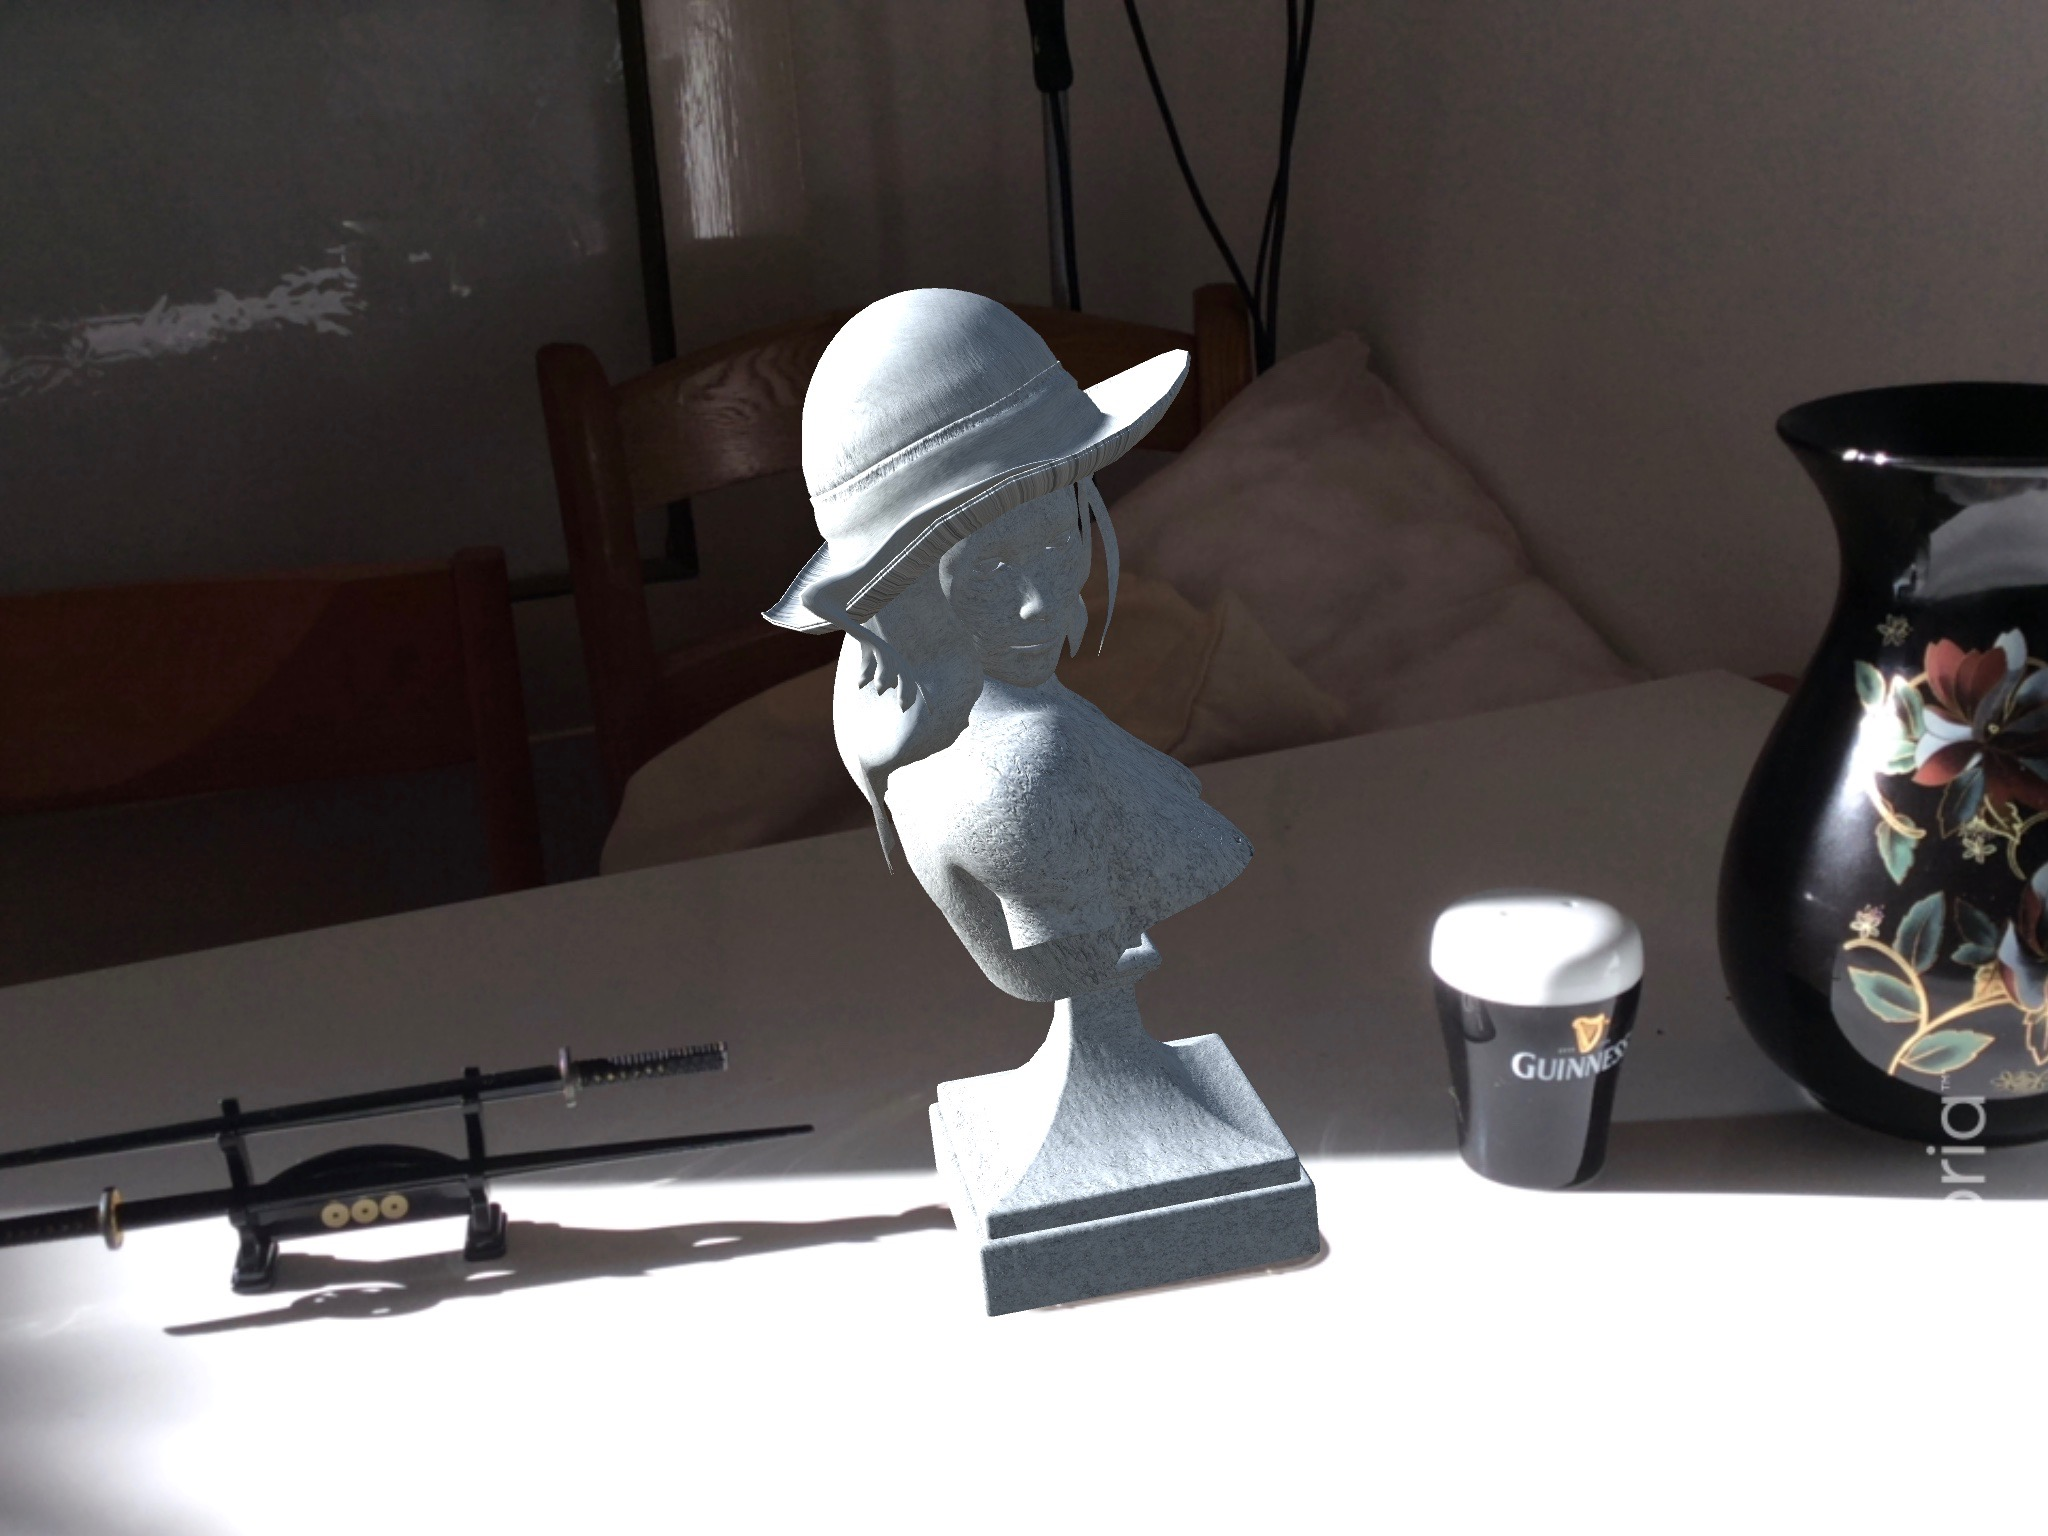
\includegraphics[width=0.6\textwidth]{Figures/realish.jpg}
\caption{Adjusted lighting, giving a more believable look}
\end{figure}
